

\documentclass[12pt,titlepage]{article}

\usepackage{graphics}

\usepackage{array}
\usepackage{color}
\usepackage{colortbl}
\usepackage{xcolor}
\usepackage{url,amsfonts,epsfig}
\usepackage[applemac]{inputenc} %comando per le lettere accentate se usate mac  
%\usepackage[T1]{fontenc}
%\usepackage[utf8]{inputenc}
\usepackage[english]{babel}
%\usepackage[latin1]{inputenc} % comando per le lettere accentate se usate pc  
\usepackage[pagebackref]{hyperref}
\hypersetup{
colorlinks=false,
allbordercolors=white
}

\begin{document}
%Code for title page
\begin{titlepage}
\centering
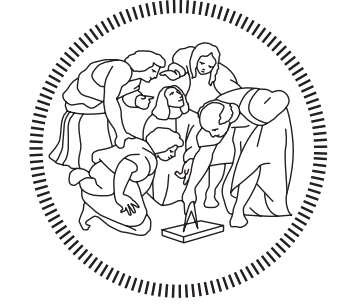
\includegraphics[width=0.4\textwidth]{Logo}\par
	{{Politecnico di Milano} \par}
	{{A.A. 2017/2018} \par}
	\vspace{1.5cm}
	
\includegraphics[width=0.9\textwidth]{LogoTravlendar}\par
	%{\Large{\textsc{{{\color{red}{ \textbf{T}rav}}lendar{\color{red}{+}}}} \\ 
		%Software Engineering 2} \par}
	\vspace{1.5cm}
	{\Huge \textbf {RASD}\par}
	{ \textbf{Requirements Analysis and Specification Document} \par}
	\vspace{1.5cm}
	{\Large\itshape Sara Pid\'o  }{\Large   {  894744}\par}
	{\Large\itshape Chiara Plizzari }{\Large   {  893901}\par}
	{\Large\itshape Giuseppe Severino }{\Large   {  898458}\par}
	\vspace{2cm}
	\vfill
	% Bottom of the page
	%{\large Document version: 3.1\par}
	\pagebreak
	{\large \today \par}
\end{titlepage}




 
\pagenumbering{roman}

%%%% Opzione per interlinea 2
%%%\baselineskip 18pt

%\maketitle

\tableofcontents
%%\listoffigures
%%\listoftables

\pagebreak

\section{Introduction} \label{introduzione}
\pagenumbering{arabic}

\subsection{Purpose} \label{sec:purpose}

\medskip
\subsubsection{Description of the RASD}\label{RASD}
RASD stands for Requirements Analysis and Specification Document.
The main goal of this document is to describe the system by clearly specifying functional and non-functional requirements in a structured though informal form in order to provide a guideline.
RASD takes into account the limits and the constraints of the problem and its possible solutions. 
It provides feedback to the customer, it serves as an input to the design specification, as a product validation check and as a contractual basis between the customer and the developer.
Therefore, RASD should be a model that is directed towards ensuring that the final system conforms to client needs.
The document is addressed to all customers and users, system and requirement analysts, developers and programmers who participate in the implementation of the requirements, testers and project managers.

\subsubsection{Purpose of the application}\label{RASD}
The application should be useful for busy people that have to travel from a place to another one because of their engagements. It helps people by organizing their own calendar: it finds the best solution to reach a certain place in a specific time basing on user's preferences. 
Users are able to see their meetings, their journey between them, their breaks and in every time they can modify their day calendar by modifying an activity or deleting it.

\subsection{Scope}\label{RASD}
\subsubsection{Description of the given problem}\label{RASD}
We want to create a calendar-based application which name is Travlendar+. It is a software that provides a support to everyone that has scheduling meetings at various locations. It helps the user in finding the best option to reach the destination in the optimal conditions and at a fixed time. 
Once the user has registered and has inserted time and place of his/her meetings, the system automatically computes and accounts for travel time between appointments, to make sure that the client will not be late. Moreover, the user will be warned if the location is not reachable at the allotted time. Other services are provided, such as the possibility to identify the best mobility option basing on user's preferences (preference or avoidance for a determined mean) and on external conditions (weather, strikes), the opportunity to buy public transportation tickets and to locate the nearest bike of a bike sharing system or the nearest car of a car sharing system. It is also possible to select combinations of transportations means that minimize carbon footprint and to specify the maximum walking distance.
Thanks to this application the users can also organize in a customizable way their break time between an appointment and one other, for example by managing a flexible lunch. 

\subsubsection{Actual system}\label{RASD}
Even if there already exist applications that allow users to find the best travel solution, this is a new kind of application for the innovative idea of managing the time. Therefore, we assume that the whole system will be created by new.
However, the application will exploit applications or websites to allow the user to buy transportation's tickets and to use sharing services. Moreover, it will profit by these websites to have real-time news on weather, strikes...

\subsubsection{Goals}\label{RASD}
\begin{itemize}

\item [{[G\textsubscript{1}]}]	A user should be able to go to a meeting.
\item [{[G\textsubscript{2}]}]	A user should be able to know if he/she cannot arrive on time to a meeting.
\item [{[G\textsubscript{3}]}]	A user should be able to have a break that has a minimum duration between two meetings.
\item [{[G\textsubscript{4}]}]	The time or the location of a meeting can be modified.

\item [{[G\textsubscript{5}]}]  A user should be able to unsay  a meeting.
\item  [{[G\textsubscript{6}]}] A user should be able to have some preferences for the trip.
\begin{itemize}
\item [{[G\textsubscript{6.1}]}]	A user should be able not to use some travel means.
\item [{[G\textsubscript{6.2}]}]	A user should be able not to walk more than a specific distance.
\item [{[G\textsubscript{6.3}]}] A user should be able to minimize carbon footprint when he/she goes to a meeting.
\end{itemize}
\item [{[G\textsubscript{7}]}] A user should be able to know every possible option to go to a meeting with different travel means in order to choose the suitable one.
%\item [{[G\textsubscript{7}]}]	 provide constraints on different travel means;
\item [{[G\textsubscript{8}]}]	A user should be able to buy public transportation tickets or day/week/season pass basing on his/her needs.
\item [{[G\textsubscript{9}]}]	A user would like to see on Tripadvisor advised places for his/her breaks.
\item [{[G\textsubscript{10}]}]	A user would like to locate the nearest vehicle of a vehicle sharing system if he/she wants to use that type of travel means.
\item [{[G\textsubscript{11}]}]	A user would like to have real-time news on strikes, weather and traffic.

 \end{itemize}
\subsubsection{Actors}\label{RASD}
There are two types of actors:
\begin{itemize}
\item Visitors: people that download the application and that are not registered in the system but they have free access to the login page, the sign-up page.
\item Registered users: they can see all the pages available to visitors and after successful login, they can take advantage of all the services of the application.

\end{itemize}


\subsection{Definitions, acronyms, abbreviations}\label{RASD}
\subsubsection{Definitions}\label{RASD}
\begin{itemize}
\item Visitor: a person that is not registered yet, but has the access to the application's information. 
\item	Registered user: a person that is logged in the system and can create meetings.
\item	Activity: an event that happens in the real world and that could be a meeting or a break.
\item	Meeting: an activity among the registered user and other people. It can be created, modified and deleted by the meeting's creator. 
\item	Break: an activity that a registered user can insert in order to manage it in a customizable way.
\item Trip: it indicates the route and the travel means chosen, based on user's preferences.
\item Global preferences: they are global attributes that registered users can modify and those are valid for all trips (i.e. minimize carbon footprint).
\item	Creation screen: the screen of the application in which the registered user create a meeting or a break and enters its related details.
\item Blocked travel means: it is a travel means that the user has selected as unwanted.
\item Warning: a message directed to the user that arrives to him in form of a notification and can be shown on the application screen. It is generated by the system when there are some impediments for a trip (bad weather, strikes, traffic...) or when there are some problems (invalid data during the registration process or during the creation of an activity etc).
\end{itemize}
\subsubsection{Acronyms}\label{RASD}
\begin{itemize}
\item	RASD: Requirements Analysis and Specification Document
\end{itemize}
\subsubsection{Abbreviations}\label{RASD}
\begin{itemize}
\item	Gi: i-goal
\item	Ri: i-requirement
\item	Di: i-domain assumption
\item Ai: i-assumption 
\item DEi: i-dependency
\item Ci: i-constraint
\item Ui: i-use case
\end{itemize}
\subsection{Revision history}\label{RASD}

\subsection{Reference documents}\label{RASD}
\begin{itemize}
\item Specification Document: Mandatory project assignment;
\item IEEE Std 830-1998 IEEE Recommended Practice for Software Require-
ments Specifications;
\item``Alloy come strumento di analisi e progettazione di sistemi software" (graduate thesis of Claudio Vallorani);
\item Alloy Language Reference;
\item Example RASD of previous years;
\item ``Introduzione all'arte della composizione tipografica con LATEX".
\end{itemize}


\subsection{Document structure}\label{RASD}
This document is structured as follows:
\paragraph{Section 1: Introduction}
In this section it is described the purpose of this document, the main goals of the given problem and a brief description of its main characteristics. 
\paragraph{Section 2: Overall Description}
It provides further information about the application with a summary of major functions and it states all the assumptions and the constraints.
\paragraph{Section 3: Specific Requirements}
In this part we include more details about the requirements.
\paragraph{Section 4: Formal Analysis using Alloy}
This section provides the Alloy model and all the proves that it supplies.
\paragraph{Section 5: Effort spent}
Here are reported the information about the hours of work spent by each member of the group by doing this project.
\paragraph{Section 6: References}
\pagebreak

\section{Overall description}\label{sec:crit}

%Riprendiamo quanto visto nella sezione~\ref{sec:mod1}, bla bla...
\subsection{Product perspective}\label{sec:mod1}
Our application requires a smartphone (iOs/Android) to be executed and it requires an internet connection in order to benefit from the application's main services.
It also requires an active GPS connection to identify the user's position. 
Travlendar+ is similar to other pre-existing applications that compute the best route with the best means to reach a specific location (e.g. Moovit), and like them, it is supported with updated timetables of all the travel means and with an estimation of travel time. 

\begin{figure}
\subsubsection{Class diagram}\label{sec:mod1}
\centering
\makebox[\textwidth]{\includegraphics[scale=0.4]{"Class Diagramv2"} }
\caption{Class Diagram}
\end{figure}


 \clearpage
\newpage
 \begin{figure}
\subsubsection{Statechart diagram }\label{sec:mod1}
\centering
\makebox[\textwidth]{\includegraphics[scale=0.6]{"Statemachine1"}  }
\caption{Login}
\par
\makebox[\textwidth]{\includegraphics[scale=0.45]{"Statemachine2"} }
\caption{Application}
\end{figure}

\clearpage
\newpage
 
\pagebreak 
\subsection{Product functions}\label{sec:mod1}
We already identified the goals that characterized functionalities of Travlendar+. Instead, in this section, we offer a specific list of the main features of the application in order to explain better its utility. 

\paragraph{Offline mode}
Travlendar+ could be used in offline mode simply as a basic calendar. Users' can visualize on the main screen all their activities for the day, by clicking them they can see all details about the location and the time. In this mode, it isn't possible to see the map with the computed trips. Users' can also insert new activities by pressing the plus button, whereas if they click on the calendar icon, they are able to visualize the whole calendar. 

\paragraph{Map}
The application offers the possibility to visualize the map of the interested area. If there is any activity saved in the calendar for the current day, an indicator is shown in its location. On the map, a blue line highlights the trip between the different meetings of the day. By pressing an activity appears also the chosen path to reach it from the actual location. By pressing "GO" it can be visualized the whole path of the day.

\paragraph{Personalization}
Travlendar+ offers a lot of options that can be customized, for example, the user can:
\begin{itemize}
\item{specify a minimum duration of the lunchtime;}
\item {specify everyday lunchtime;}
\item{activate or deactivate travel means;}
\item{insert the maximum walking distance;}
\item{select combinations of transportation means that minimize carbon footprint;}
\item{deactivate public transportation in a certain time zone.}
\end{itemize}

\paragraph{The best route's computation}
Once a meeting is created Travlendar+ suggests the best route between the previous, the current and the next activity of the day that satisfies the constraints of the user. If the user is not satisfied with the proposed trip, he/she can choose another one between those suggested by the app.

\paragraph{Real-time information}
Every time the system is updated with the information about the traffic, the weather, strikes etc. The user can either receive the respective notification or visualize all the warnings on the main screen. All these warnings influence the choice of the travel means for the trip. 


\paragraph{Possible future implementations} 
There are some interesting ideas that can be applied to Travlendar+ in the near future. Here we make some examples.
\begin{itemize}
\item Users can specify in the calendar also how they want to spend their break time. If they have a lot of time between an appointment and another, they can decide to have an "entertainment break". In this case they will select it, and Travlendar+ will inform them of the entertainment activities near the meeting point (i.e. cinemas, museums...).
\item The external websites on which Travlendar+ deals could be integrated. In this way users are not redirected to other websites, but they can manage all from the same application. For example, they would not need to use the Trenitalia's website to buy train tickets (this implies that they also have to register and insert their payment method to other websites ecc..), or they will not need to install other applications to use a vehicle-sharing service.  In order to do this, it will be requested to the user during the registration process to insert the payment data. Since the payment data need more protection, it could be implement a system that sends the password to the user at the moment of the registration to guarantee more security. 
\item Users can invite friends to an event at which they participate.  
\item Users can ask some friends that participate at the same meetings to share part of the trip with them. 

\end{itemize}

\subsection{User characteristics}\label{sec:mod1}
Travlendar+ has no specific user target: everyone, that is able to use a device with an internet connection, can take advantage of this new type of calendar application.
However, the user that we expect to benefit most is a busy person who wants to organize his/her daily activities in the best way, finding the fastest and the most comfortable way to travel between two activities and to reach the destination on time.
To own a personal calendar, the user must have a device with an internet connection and register with all necessary data or sign in with Facebook or Twitter.

\subsection{Assumptions, dependencies and constraints}\label{sec:mod1}
\paragraph{Assumptions}
\begin{itemize}
%\item To become a registered user, a visitor must either insert name, surname, username, password, email, address, date of birth, telephone number or sign up with Facebook or Twitter.
%\item A visitor can see only the login and registration page.
%\item Password must be at least 8-characters long for security reason.
%\item To log in a registered user must provide the username and the password associated with him/her.
%\item A registered user can create an unlimited number of meetings.
%\item The calendar for each user is unique.
%\item When meetings overlap, or they can not be reached in the allotted time, a warning is created in order to make the user modify meetings or trips.
%\item In order to buy public transportation's tickets or to use vehicle sharing systems, the user is redirected to websites/apps that provide those services.
%\item Warnings are visualized inside the meeting's information screen.
%\item When a warning is generated, a notification is sent to the user's device.
%\item If the trip chosen is expected to be done by a vehicle sharing system, we assume that in the starting location there are some vehicles available.
%\item If there are some problems with a trip, and in consequence it is unavailable, a warning is sent to the user. The user can close the warning, and the application will automatically open the screen with the choice of the trip in order to let him choose another one.
%\item In the section ``My Account'' a user can modify personal data and can express global preferences (e.g. activate/deactivate each travel means, specify the minimum lunch duration).
%\item In the creation screen, a user must specify the type of activity to be added (break or meeting).
%\item To create a meeting, users must insert name, location, date, starting/ending hours. Optionally they can also insert a brief description.
%\item The application is real-time informed about traffic, weather and strikes.
\item [{[A\textsubscript{1}]}]  Accurate registered user's location is known by GPS.
\item [{[A\textsubscript{2}]}] The user knows the right details about the activities.
\item [{[A\textsubscript{3}]}] The public transportations are always in time.
\item [{[A\textsubscript{4}]}] The external third part services (e.g. vehicle sharing systems, google maps, travel means' websites ecc...) work correctly.
\item [{[A\textsubscript{5}]}] The news about the traffic, the weather and strikes are correct.
\end{itemize}

\paragraph{Dependencies}
\begin{itemize}
\item[{[DE\textsubscript{1}]}]  The application depends on external application and websites for some services, such as: the purchase of public transportation's tickets, the use of vehicle sharing systems. 
\item [{[DE\textsubscript{2}]}] The application bases on some other services like google maps, meteo services and traffic services and uses the received information to guarantee its services.
\end{itemize}

\paragraph{Constraints}
\begin{itemize}
\item [{[C\textsubscript{1}]}] Travlendar+ requires a smartphone or a tablet with internet connection in order to offer its functionalities.
\item [{[C\textsubscript{2}]}] Travlendar+ needs a GPS service to find the correct location of the user.

\end{itemize}

\begin{figure}
\subsection{The World and The Machine}\label{sec:mod1}
\begin{flushleft}
In order to analyze Travlendar+, we would like to consider The World and Machine model. It was presented in 1995 by M.Jackson and P.Zave and it is useful to identify requirements. In this way, we can divide them into three parts: the portion of the real-world that interact with the application (the World), the portion of the system to be developed (the Machine) and the intersection between the two (Shared phenomena), that are all world information known or managed by Travlendar+.
We insert also an example of these components, even if it is not complete.
\end{flushleft}

\centering
\makebox[\textwidth]{\includegraphics[scale=0.65]{"worldAndMachine"} }
\end{figure}

\pagebreak
\section{Specific requirements}\label{sec:crit}

\subsection{External interface requirements}\label{sec:mod1}
\subsubsection{User interfaces}\label{sec:mod1}
Our application has been designed to be used through a smartphone or a tablet.
The following mock-ups show the screens of the main features offered by the smartphone version. 

\begin{figure}
\centering
\makebox[\textwidth]{\includegraphics[scale=0.15]{"mockup login"} }
\caption{This is the login screen that appears when a visitor opens the application.}
\end{figure}
\clearpage
\newpage

\begin{figure}
\centering
\makebox[\textwidth]{\includegraphics[scale=0.15]{"mockup meeting"} }
\caption{This is the main screen that appears when a registered user logs in.}
\end{figure}
\clearpage
\newpage

\begin{figure}
\centering
\makebox[\textwidth]{\includegraphics[scale=0.15]{"mockup options"} }
\caption{To modify user's preferences, to go to the map screen and for other features, the user should tap on the menu icon on the left top corner.}
\end{figure}
\clearpage
\newpage

\begin{figure}
\centering
\makebox[\textwidth]{\includegraphics[scale=0.15]{"mockup add activity"} }
\caption{This is the screen that allows the registered user to add a new activity, by specifying its type and details.}
\end{figure}
\clearpage
\newpage

\begin{figure}
\centering
\makebox[\textwidth]{\includegraphics[scale=0.15]{"mockup modify activity"} }
\caption{This is the screen that is shown to the registered user when a tap on an existing activity is performed. This allows the registered user to modify or remove the entire activity. }
\end{figure}
\clearpage
\newpage

\begin{figure}
\centering
\makebox[\textwidth]{\includegraphics[scale=0.15]{"mockup trip selection"} }
\caption{This is the screen that shows the various trip options suggested by Travlendar+ after that the registered user has inserted a new activity. }
\end{figure}
\clearpage
\newpage

\begin{figure}
\centering
\makebox[\textwidth]{\includegraphics[scale=0.15]{"mockup map"} }
\caption{This is the screen that shows the map with all activities of the current day. Moreover, it shows the different trips that the user should do. The activities are shown through a tap on the pointer.}
\end{figure}
\clearpage
\newpage

\subsubsection{Hardware interfaces}\label{sec:mod1}
The application does not require any hardware interface. 

\subsubsection{Software interfaces}\label{sec:mod1}
Travlendar+ does not provide for itself the possibility to directly buy public transportation's tickets and the possibility to use sharing systems, but redirects the user to the corresponding website or, if it's already installed in the device, to the corresponding app.

\subsubsection{Communication interfaces}\label{sec:mod1}
The application needs an internet connection on the device in order to receive real-time information about traffic, strikes and weather. Furthermore, it's required also for the communication with third-party services that are provided in Travlendar+. 





\subsection{Functional requirements}\label{sec:mod1}

\paragraph{Prerequisites}
\begin{itemize}
\item[{[R\textsubscript{1}]}] The system should allow the visitor to begin the registration process by asking him/her all mandatory data: name, surname, date of birth, email, username, password.
\item[{[R\textsubscript{2}]}] The system should be able to extract data from Facebook or Twitter if the visitor signs in with that application.
\item[{[R\textsubscript{3}]}] The system must not allow a registered user to perform registration process.
\item[{[R\textsubscript{4}]}] The system must allow visitors only to see the login page and the registration form.
\item[{[R\textsubscript{5}]}] The system should allow only registered users to log in.
\item[{[R\textsubscript{6}]}] Username and password inserted must be correct to perform the login.
\paragraph{Requirements}
%\item[\textbf{ {[G\textsubscript{1}]}}]	\textbf{	Users should be able to sign up into the application.}
%\begin{itemize}
%\item[{[R\textsubscript{1}]}] The system should allow the visitor to begin the registration process by asking him/her all mandatory data: name, surname, date of birth, email, username, password.
%\item[{[R\textsubscript{2}]}] The system should be able to extract data from Facebook or Twitter if the visitor signs in with that application.
%\item[{[R\textsubscript{3}]}] The system must not allow a registered user to perform registration process.
%\item[{[R\textsubscript{4}]}] The system must allow visitors only to see the login page and the registration form.

%\item[{[D\textsubscript{1}]}] The username must be unique.
%\item[{[D\textsubscript{2}]}] The password must be at least of 8 characters.
%\item[{[D\textsubscript{3}]}] The email address must be correct.
%\end{itemize}
%\item[\textbf{ {[G\textsubscript{2}]}}]	\textbf{	Users should be able to log into application.}
%\begin{itemize}
%\item[{[R\textsubscript{1}]}] The system should allow only registered users to log in.
%\item[{[R\textsubscript{2}]}] Username and password inserted must be correct to perform the login.
%\item[{[R\textsubscript{3}]}] Visitors cannot access the calendar and to the map without login.
%\end{itemize}
\item[\textbf{ {[G\textsubscript{1}]}}]	\textbf{	A user should be able to go to a meeting.}
\begin{itemize}
%\item[{[R\textsubscript{1}]}] The system should allow only registered users to create activities.
\item[{[R\textsubscript{1}]}] The system should allow registered users to create meetings.
%\item[{[R\textsubscript{2}]}] Users must be logged in the application.
\item[{[R\textsubscript{2}]}] Users must complete the form by filling the mandatory fields and confirm the creation.
%\item[{[R\textsubscript{3}]}] Users must specify the type of activity (meeting or break).
%\item[{[R\textsubscript{4}]}] The system should provide different form based on the type of the activity.

%\item[{[D\textsubscript{1}]}]  Time must be included between 00.00 and 23.59.
%\item[{[D\textsubscript{2}]}]  Dates must be specified in the form of dd/mm/yyyy.
%\item[{[D\textsubscript{3}]}]  Dates must be fixed in the current day or after.
%\item[{[D\textsubscript{4}]}] Days must be included between 1/01 and 31/12
\end{itemize}
\item[\textbf{ {[G\textsubscript{2}]}}]	\textbf{	A user should be able to know if he/she cannot arrive on time to a meeting.}
\begin{itemize}
\item[{[R\textsubscript{3}]}] The system should be able to calculate necessary time for each trip option.
\item[{[R\textsubscript{4}]}]  The system should be able to notify the user if there is not any option that makes him/her arrive on time.
\item[{[R\textsubscript{5}]}] Users should be able to close the warning.
\end{itemize}

\item[\textbf{ {[G\textsubscript{3}]}}]	\textbf{	A user should be able to have a break that has a certain duration between two meetings.}
\begin{itemize}
\item[{[R\textsubscript{6}]}]  The system should allow the user to create an activity with type "Break".
\item[{[R\textsubscript{7}]}]  The system should allow the user to specify the minimum duration of the break.
\item[{[R\textsubscript{8}]}]  The system should be able to provide a solution to have a break if a user specifies it.
\end{itemize}
\item[\textbf{ {[G\textsubscript{4}]}}]	\textbf{	The time or the location of a meeting can be modified.}
\begin{itemize}
%\item[{[R\textsubscript{1}]}]  Users should be registered and logged in.
\item[{[R\textsubscript{9}]}] The activity that the user wants to modify must be already created.
\item[{[R\textsubscript{10}]}] Users must confirm the modification to conclude the process.
\item[{[R\textsubscript{11}]}] Modified data will not be available any more after the update.
\end{itemize}
\item[\textbf{ {[G\textsubscript{5}]}}]	\textbf{	A user should be able to unsay a meeting.}
\begin{itemize}
\item[{[R\textsubscript{12}]}] The activity that the user wants to delete must be already created.
\item[{[R\textsubscript{13}]}] Users must confirm the elimination of the activity.
\item[{[R\textsubscript{14}]}] Activity will not be seen on the calendar and on the map.
\item[{[R\textsubscript{15}]}] Deleting process is not reversible.
\end{itemize}
\item[\textbf{ {[G\textsubscript{6}]}}]	\textbf{A user should be able to have some preferences for the trip.}
\begin{itemize}
\item[{[R\textsubscript{16}]}]  The system must keep track of user's preferences.
\item[{[R\textsubscript{17}]}] A travel means that should be deactivated must be active.
\item[{[R\textsubscript{18}]}] A travel means that should be activated must be non-active.
\item[{[R\textsubscript{19}]}]  The system should not allow users to deactivate all travel means otherwise the computation of the trip is not possible.
\item[{[R\textsubscript{20}]}]  The system should be able to calculate the carbon footprint and to minimize it.
\item[{[R\textsubscript{21}]}]  The system should not allow users to impose constraints on deactivated travel means.
%\item[{[R\textsubscript{7}]}]  The system should be able to provide a solution to have a break if a user specifies it.
%\item[{[D\textsubscript{1}]}] Travel means must be available in the reality.
\end{itemize}

%\item[{[D\textsubscript{1}]}] Travel means must be available in the reality.
%\item[{[D\textsubscript{2}]}] Constraints must be reasonable.
\item[\textbf{ {[G\textsubscript{7}]}}]	\textbf{	A user should be able to know every possible option to go to a meeting with different travel means in order to choose the suitable one.}
\begin{itemize}
\item[{[R\textsubscript{22}]}]  The system should be able to compute the different routes with several travel means.
\item[{[R\textsubscript{23}]}] The system should be able to know the activities of the day and provide a route between them.
\item[{[R\textsubscript{24}]}] The system should be able to calculate the necessary time for each trip option and shows it to the user.
\end{itemize}

\item[\textbf{ {[G\textsubscript{8}]}}]	\textbf{	A user should be able to buy public transportation tickets or day/week/season pass basing on his/her needs.}
\begin{itemize}
\item[{[R\textsubscript{25}]}]  The system should be able to open the application or the website of the service that provides that type of trip.
\item[{[R\textsubscript{26}]}] Users must confirm if they want to open an external application.
%\item[{[D\textsubscript{1}]}]  The chosen travel means must provide a web service.
\end{itemize}
\item[\textbf{ {[G\textsubscript{9}]}}]	\textbf{	A user would like to see on Tripadvisor advised places for his/her breaks.}
\begin{itemize}
\item[{[R\textsubscript{27}]}]  The system should be able to open the application or the website of Tripadvisor.
\item[{[R\textsubscript{28}]}] Users must confirm if they want to open an external application.
\end{itemize}

\item[\textbf{ {[G\textsubscript{10}]}}]	\textbf{	A user would like to locate the nearest vehicle of a vehicle sharing system if he/she wants to use that type of travel means.}
\begin{itemize}
\item[{[R\textsubscript{29}]}]  The system should be able to open the application or the website of the service.
\item[{[R\textsubscript{30}]}] Users must confirm if they want to open an external application.
%\item[{[D\textsubscript{1}]}]  The chosen service must have an application or a website.
\end{itemize}

\item[\textbf{ {[G\textsubscript{11}]}}]	\textbf{	A user would like to have real-time news on strikes, weather and traffic.}
\begin{itemize}
\item[{[R\textsubscript{31}]}] The system should be informed about weather, strikes and traffic in real time exploiting other systems.
\item[{[R\textsubscript{32}]}]  The system should be able to notify the user if there are problems that can change his/her trips.
\item[{[R\textsubscript{33}]}] Users should be able to close the warning.
\item[{[R\textsubscript{34}]}] Users should be able to change the trip.
\item[{[R\textsubscript{35}]}]  The system should be able to open again the screen with the different trip options
%\item[{[D\textsubscript{1}]}]  The real-time information must be correct and provided by reliable sites.
\end{itemize}
\end{itemize}
\subsubsection{Scenarios}\label{sec:mod1}
\paragraph{Scenario 1} 
Dybala is a very busy football player that lives in Turin. Tomorrow morning he is going to have an important meeting with one of the main sponsor of the Juventus team, the Adidas, in Milan, and in the evening he has the Champions League's final. It is the most important match of the year, so he needs to organize his day at the best! He decides to use Travlendar+. He inserts the two activities in the list of meetings: ``Meeting with Adidas", on 20th of May, from 11 am to 1 pm, in Corso Buenos Aires 40 (Milan) and ``Match prep for the Final", on 20th of May, from 3 pm to 7 pm, at the Allianz Stadium (Turin). Since he wants to preserve energies for the Final, he selects "Walking" and "Bike" as blocked travel means in the Preferences' area. The application suggests him a trip with the train from Turin to Milan in the early morning because the estimated time for the route by car or taxi is reported to be slower due to the traffic. The application redirects him to the Trenitalia's website to buy the ticket. Then, for coming back, Travlendar+ suggests him to take a taxi because public transport timetables for the given time are not convenient. 

\paragraph{Scenario 2}
Giuseppe is a student at Politecnico of Milan. In view of the exams session, he has not much time but he does not want to give up a good lunch with his friends. Therefore, he specifies in the "My Account" section of Travlendar+ that every day he needs at least 30 minutes free to have a comfortable lunch between 11.30 am and 2.30 pm. He inserts the schedule of all his lessons. After having inserted the Formal Languages and Compilers' lesson of Wednesday, a warning appears to report an overlap with the fixed time reserved for the lunch. He can ignore the warning and decide what he prefers to do.

\paragraph{Scenario 3}
Carlo Cracco is a famous chef that has two restaurants in Milan. He would like to open a new restaurant in Verona. So he has to go to Verona to search for a place that can be restored as he likes and to meet architects and designers to decide all details of the new restaurant. He would like to have a coffee break between the afternoon appointments to restore himself. Therefore he uses Travlendar+ to organize the full day. He inserts all the meetings and he also inserts the coffee break: pressing the plus symbol on the main screen, Carlo selects the type ``Break'', he inserts the minimum duration for the break and he is readdressed to the website ``TripAdvisor''. In this way, the chef can see what coffee is opened near the two appointments that he has before and after the break and he can choose the best one.

\paragraph{Scenario 4}
Lorenzo Fragola is a young boy with a strong passion for singing, so he decides to go to an audition for XFactor, the most famous music talent show in Italy. The audition will take place on the 30th of July in Milan, at Arena Civica. Lorenzo lives in Catania and decides to use Travlendar+ to program the trip for the audition. He inserts the meeting in the system, with the date, the location and the time, and visualizes the trip. The two available means suggested by the application are the train, which takes 13 hours, and the car, which takes 14 hours. Since both take too long, he decides to organize himself the trip with the plane. Once he will be in Milan, he will use the application to go to the Arena Civica. The trip suggested is by autobus from the airport to the railway station, and then by metro to the Arena. Unfortunately, one week before the audition, a warning appears on his phone: on the day of the audition, there will be a strike of ATM! At first Lorenzo is a little bit worried, but immediately sees that Travlendar+ has suggested him an alternative trip by car (taxi or car sharing) from the railway station to the Arena. He will choose at that day the best option. When the moment arrives, he selects car sharing as favourite means, and the application redirects him on the play store to download the Enjoy's application (the car-sharing service). Through Enjoy's application, he can see that there is a car near the station and he can book it.

\paragraph{Scenario 5}
Travlendar+ has become a very well known application. A lot of people start to use it and find Travlendar+ the most useful application of 2017. 
Also, the USA president has become curious because of the fame of this new type of smart calendar. He decides to try it: he has an iPhone X and he goes to the AppStore and installs it.
Once it is installed, Trump opens it and he finds out that he has to sign in. He clicked the "Sign in" button and a new screen appears. 
He has to insert a lot of personal information: name Donald, surname Trump, date of birth 14/06/1946, address 1600 Pennsylvania Ave NW, Washington, username Tump, password ******** and at the end the telephone number +1 202-456-1111.
Once he finishes compiling, he clicks "Sign in" and the screen for the registered users appears: there is the screen with the schedule of the day that is obviously empty for new users.

\paragraph{Scenario 6}
Mr. Bean is a very busy man that uses Travlendar+ to manage his great number of appointments. Once he inserts a work meeting in the morning between 10.00 and 12.00, he decides to go with his loved car. After that, he knows that he has to be present to a ceremony for his teddy bear's birthday that should start at 11.45 a.m.. This cannot be possible!!! Travlendar+ notifies him with a warning that there is an overlap between two appointments. Therefore Mr. Bean closes the warning and decides to go out of the conference before to arrive on time at the birthday.
Mr. Bean is very excited and decides to have a stop in a toy shop to buy a present. So he inserts in the application the new activity but there is another problem. With a warning, Travlendar+ warns him that if he wants to arrive on time at the ceremony, he cannot go to the shop. Hence he does not confirm the creation of the activity.

\paragraph{Scenario 7}
Leonardo DiCaprio is a famous actor that has always been active in fighting climate change. To raise awareness among the people about the environmental problems, he has the idea to live stream one of his ordinary day to show people the importance of using means of transport that minimizes carbon footprint. 
Leonardo decides to use Travlendar+ in order to arrange his trips in the day. Once the application is installed and he creates his personal account, Leonardo inserts three activities (all in New York) to be performed during the day. The application now suggests the ideal route that minimize travel durations, but in order to pursue his goal Leonardo enter the "My Account" section of the app and then he enables, in the preferences' area, the option "Minimize footprint". The route suggested by the application seems to be more eco-friendly, for example, Travlendar+ proposes to him to rent a bike or to use a service of electric car sharing.

\paragraph{Scenario 8}
Claire is going to have a marry of her best friend on Sunday morning. Since after the ceremony there will be a big party with food and drink, she decides not to drive. To discover the best option to reach the church, she uses Travlendar+. The application suggests her to take the metro and then to walk for ten minutes from the underground station to the destination. It's all perfect for her, but unfortunately, she wakes up on Sunday morning and it is raining. She can not afford to walk under the rain because she has just gone to the hairdresser! She immediately logs in to the application to check an alternative trip. Travlendar+, that has an updated weather forecast, has already changed the trip: it suggests her to take the tram once exited from the underground station instead of walking. She notices looking at the tram schedule in the activity's details that she will not take much more to go there with this alternative because trams of line 34 stops every 13 minutes. She will reach the destination in time.

\paragraph{Scenario 9}
Guglielmo is a Computer science engineer. He works for a big company: he earns a lot of money. Because he often had to move, he used a lot his car. Guglielmo was very reckless, in fact, he went on taking fines, even very expensive. He didn't care about it. But once the police gave him another big fine and withdrew his driving license and confiscate his car.
Since he lives in Milan and he hates public transports, he decides to try the application Travlendar+. He enrolls in the app and in the section "My Account" he deactivates every public transportations and sharing cars. He has to go to work: when the trip is suggested, he presses on bike sharing's option because he really love the speed and he has a lot of time to reach the location. Guglielmo is redirected to the Ofo's application and from that application, he can see where is the nearest bike. Finally, he can go fast without taking any fine!




\pagebreak
\subsubsection{Use case diagrams}\label{sec:mod1}
\begin{flushleft}
\textbf{Registration} 
\end{flushleft}

\begin{tabular}{cp{10cm}} 
Use case ID& {[U\textsubscript{1}]}\\ \hline
Actor&Visitor\\ \hline 

Input condition&NULL \\ \hline
Event flow&The registration's process is: \begin{enumerate}
\item The visitor tap on ``sign up" on the home page to start the registration process.
\item The visitor fills in at least the mandatory fields, that are: name, surname, username, password, email, address, date of birth. The non-mandatory field is the telephone number.
\item The visitor tap on ``ok".
\item The application saves the data and redirects him to the home page where he can proceed to the login.
\end{enumerate} \\ \hline
Output condition&Registration process is completed. The visitor becomes a registered user. \\ \hline
Exception& The possible exceptions are:
\begin{enumerate}
\item The visitor is already a registered user.
\item The visitor fills one or more fields with invalid information.
\item The visitor chooses an already existent username.
\item The visitor inserts an email that is already associated with another user.
\end{enumerate} 
In case of an exception the invalid fields are coloured with red. The visitor can't press ``ok" until all fields are correctly filled.\\ \hline \

\end{tabular}

\pagebreak

\begin{figure}
\centering
\makebox[\textwidth]{\includegraphics[scale=0.65]{"UseCase Registration"} }
\caption{Use case of the registration process}

\end{figure}

\begin{figure}
\centering
\makebox[\textwidth]{\includegraphics[scale=0.64]{"SequenceDiagram Registration"} }
\caption{Sequence diagram of the registration process}
\end{figure}

\clearpage
\newpage


\begin{flushleft}
\textbf{Login} 
\end{flushleft}

\begin{tabular}{cp{10cm}} 
Use case ID& {[U\textsubscript{2}]}\\ \hline
Actor&Visitor, registered user\\ \hline 

Input condition&The user is on the homepage.\\ \hline
Event flow&The login's process is:\begin{enumerate}
\item The registered user fills the fields ``username" and ``password" with her/his username and password. Alternatively, a simple visitor can tap on "Login with Facebook" or "Login with Twitter" in order to login directly without having completed the registration process.   
\item If the access is not with Facebook or Twitter, after having inserted the username and password the registered user must tap on ``Login".

\end{enumerate} \\ \hline
Output condition& Travlendar+ verifies user's credentials (either they have been directly inserted by the user or obtained through Facebook or Twitter) and if they are correct shows the main screen with the map with the activities.
\\ \hline
Exception& The possible exceptions are:
\begin{enumerate}
\item The user inserts an incorrect username or password.
\item The user's data obtained by Facebook or Twitter are invalid.
\end{enumerate} 
In both the cases, the user is notified with an error message and invited to try again.\\ \hline \

\end{tabular}


\pagebreak
\begin{figure}
\centering
\makebox[\textwidth]{\includegraphics[scale=0.7]{"UseCase Login"}  }
\caption{Use case of the login process}

\end{figure}
\begin{figure}
\centering
\makebox[\textwidth]{\includegraphics[scale=0.55]{"SequenceDiagram Login"} } 
\caption{Sequence diagram of the login process}
\end{figure}

\clearpage
\newpage
 
\begin{flushleft}
\textbf{New activity}
\end{flushleft}


\begin{tabular}{cp{10cm}} 
Use case ID& {[U\textsubscript{3}]}\\ \hline
Actor&Registered user\\ \hline 
Input condition&The registered user is already logged into Travlendar+.\\ \hline
Event flow&The process for the creation of a new activity is: \begin{enumerate}
\item The registered user tap on the plus icon (``new activity button").
\item Travlendar+ shows a new page with the form, and the creation process starts. The user is required to specify the type of activity (meeting or break) and to insert all the attributes about the activity, such as name, date, time, location and favourite means. If the activity is of type ``break", the registered user must also specify a minimum duration of the activity.
\item The registered user tap on ``ok".
\end{enumerate} \\ \hline
Output condition& Travlendar+ redirects the registered user on the main screen. On the map is appeared the new activity on its location. 
\\ \hline
Exception& The possible exception is that the user does not fill a mandatory field or fills it with invalid data. In such cases, the invalid fields are coloured with red. The user must insert the correct data in order to complete the creation of the activity.

\\ \hline \

\end{tabular}
\pagebreak

\pagebreak
\begin{figure}
\centering
\makebox[\textwidth]{\includegraphics[scale=0.5]{"UseCase Creation of an activity"}  }
\caption{Use case of the creation of an activity}
\end{figure}
\begin{figure}
\centering
\makebox[\textwidth]{\includegraphics[scale=0.45]{"Sequence createActivity"} } 
\caption{Sequence diagram of the creation of an activity}
\end{figure}

\clearpage
\newpage

\begin{flushleft}
\textbf{Modify activity}
\end{flushleft}

\begin{tabular}{cp{10cm}} 
Use case ID& {[U\textsubscript{4}]}\\ \hline
Actor&Registered user U \\ \hline 
Input condition&U is the creator of the event A and is logged in.\\ \hline
Event flow&The process for the modification of a new activity is: \begin{enumerate}
\item U taps on the activity A on the map (coloured with blue if A is a meeting, with red if A is a break), in the section ``My activities" or in the main screen with the activity of today.
\item U taps on the ``modify" symbol.
\item The application shows the screen form of the activity that contains the fields to fill with the attributes.
\item U can modify the fields by tapping on it.
\item U taps on ``ok" when he/she has completed the modification.
\item The application updates the calendar with the new information.
\item The application redirects U to the main screen. 
\end{enumerate} \\ \hline
Output condition& Travlendar+ updates the calendar with the activity modified, then redirects U on the main screen. If the location of the location has been modified, on the map on the main screen the activity appears in the new location.
\\ \hline
Exception& The possible exceptions are:
\begin{enumerate}
\item U inserts an invalid modification.
\item U does not want to apply the modifications.
\end{enumerate} 
In the first case, the invalid field is highlighted with red. In the second one, the U can tap ``cancel" when the system asks for confirmation and no changes will be made.
\\ \hline \

\end{tabular}


\begin{figure}
\centering
\makebox[\textwidth]{\includegraphics[scale=0.6]{"UseCase Modify activity"}  }
\caption{Use case of modifying an activity}
\clearpage
\newpage
\end{figure}
\begin{figure}
\centering
\makebox[\textwidth]{\includegraphics[scale=0.45]{"Sequence modifyActivity"} } 
\caption{Sequence diagram of the modification of an activity}
\end{figure}
\clearpage
\newpage

\begin{flushleft}
\textbf{Delete activity}
\end{flushleft}

\begin{tabular}{cp{10cm}} 
Use case ID& {[U\textsubscript{5}]}\\ \hline
Actor&Registered user U \\ \hline 

Input condition&U is the creator of the event A and is logged in.\\ \hline
Event flow&The elimination of an activity's process is: 
\begin{enumerate}
\item U selects the activity from the map, from the section ``My activities" or from the main screen with the activity of today.
\item U taps on ``delete". 
\item The application asks a confirm for the elimination. If U answers ``ok", the activity is deleted from the calendar.
\end{enumerate}\\ \hline
Output condition& Travlendar+ updates the calendar, in particular, it deletes the activity from the map and from the calendar.
\\ \hline
Exception& The possible exception is that U has already tapped on "delete" but he/she does not want to delete the activity. In that case he/she can tap on ``cancel" when the system asks for the confirmation.
\\ \hline \

\end{tabular}
\pagebreak 
\begin{figure}
\centering
\makebox[\textwidth]{\includegraphics[scale=0.7]{"UseCase Delete"} }
\caption{Use case of deletion of an activity}

\end{figure}
\begin{figure}
\centering
\makebox[\textwidth]{\includegraphics[scale=0.45]{"Sequence deleteActivity"} } 
\caption{Sequence diagram of deletion on an activity}
\end{figure}
\clearpage
\newpage


\begin{flushleft}
\textbf{Choose a favourite trip}
\end{flushleft}

\begin{tabular}{cp{10cm}} 
Use case ID& {[U\textsubscript{6}]}\\ \hline
Actor&Registered user U \\ \hline 

Input condition&U is the creator of the event A and is logged in.\\ \hline
Event flow&Once the activity has been created, the screen with the choice of the trip between all meetings of that day appears. U can choose one by tapping on it. \\ \hline
Output condition& Travlendar+ updates the calendar with all the details about the trip in the corresponding activities and highlights the trip between the meetings of the day in blue. 
\\ \hline
Exception& The possible exceptions are:
\begin{enumerate}
\item The trip chosen takes too much time, and U risks to not arrive in time. 
\item The trip chosen is not available because of traffic or in case of a strike. 
\end{enumerate} 
In both cases, a notification arrives on U's screen and Travlendar+ invites him/her to do another trip. \\ \hline 

\end{tabular}

\pagebreak 
\begin{figure}
\centering
\makebox[\textwidth]{\includegraphics[scale=0.65]{"UseCase Choose trip"} }
\caption{Use case of choosing the trip}

\end{figure}

\begin{figure}
\centering
\makebox[\textwidth]{\includegraphics[scale=0.65]{"Sequence chooseFavouriteTrip"} }
\caption{Sequence diagram of choosing the trip}

\end{figure}


\clearpage
\newpage
\begin{flushleft}
\textbf{Modify global preferences}
\end{flushleft}

\begin{tabular}{cp{10cm}} 
Use case ID& {[U\textsubscript{7}]}\\ \hline
Actor&Registered user U \\ \hline 

Input condition&U is logged in.\\ \hline
Event flow&Once U is on the main screen, to modify the preferences he can:
\begin{enumerate}
\item Tap on ``menu" symbol.
\item Tap on ``App preferences".
\item Tap on one of the preferences to modify it.
\end{enumerate} 
\\ \hline
Output condition& The application saves the changes. In the trips proposed to U, it will not comprehend trips with the deactivated travel means. If the option of minimizing carbon footprint is activated, Travlendar+ will propose trip with the minimum carbon footprint, and it will not exceed the minimum walking distance in finding the routes. \\ \hline
Exception& The possible exceptions are:
\begin{enumerate}
\item U wants to activate/deactivate a travel means that is already active/non-active.
\item U wants to activate/deactivate the option of minimizing the carbon footprint, but this option is already active/non-active.
\end{enumerate}
In both cases, the new change will overwrite the last one.\\ \hline 

\end{tabular}
\pagebreak 
\begin{figure}
\centering
\makebox[\textwidth]{\includegraphics[scale=0.65]{"UseCase Modify user preferences"} }
\caption{Use case of modifying user's preferences}
\end{figure}
\begin{figure}
\centering
\makebox[\textwidth]{\includegraphics[scale=0.7]{"SequenceDiagram Modify user's preferences"}  }
\caption{Sequence diagram of modifying user's preferences}
\end{figure}

\clearpage
\newpage

 \subsubsection{Traceability matrix}
\definecolor{lightgray}{rgb}{0.83, 0.83, 0.83}
\definecolor{anti-flashwhite}{rgb}{0.95, 0.95, 0.96}
\begin{tabular}{llccr}
\rowcolor{red}
Goal ID & Req ID & Assumption ID & Use case ID \\
\rowcolor{lightgray}
 G1 &R1, R2 & A2&  U3 \\
\rowcolor{anti-flashwhite}
G2 & R3, R4, R5 & A1, A3, A4, A5& -\\
\rowcolor{lightgray}
G3 & R6, R7, R8 & - & U7 \\
\rowcolor{anti-flashwhite}
G4 & R9, R10, R11 & A2 & U4 \\
\rowcolor{lightgray}
G5 & R12, R13, R14, R15 & A2& U5 \\
\rowcolor{anti-flashwhite}
G6 & R16, R17, R18, R19, R20, R21 & - &  U7 \\
\rowcolor{lightgray}
G7 & R22, R23, R24 &A4, A5& U6 \\
\rowcolor{anti-flashwhite}
G8 & R25, R26 & A4& - \\
\rowcolor{lightgray}
G9 & R27, R28 & A4& - \\
\rowcolor{anti-flashwhite}
G10 & R29, R30& A4& - \\
\rowcolor{lightgray}
G11 & R31, R32, R33, R34, R35 & A5&- 
\end{tabular}

\subsection{Performance requirements}\label{sec:mod1}
In order to guarantee the performance of our application, we have to specify:
\begin{itemize}
\item Response Time 
\item Workload
\item Scalability
\item Platform
\end{itemize}
To be reactive and able to answer to a large number of requests, we assume that the response time is close to 0 (from Jakon Nielsen book on Usability 0.1 seconds is about the limit to have the user feel that the system is reacting instantaneously), so it depends mostly on the internet connection of the platform used. 
We assume that there will be no problem with scalability even if it is a new software and it could suffer an unexpected growth in popularity and from an increase in workload.

\subsection{Design constraints}\label{sec:mod1}
In order to be compatible both with Android and iOs, the application will be developed within the following programming languages:
\begin{itemize}
\item Swift 4 (for the iOs version)
\item Java 8 (for the Android version)
\end{itemize}
We have chosen to use the last version of the programming languages to increase robustness and stability of the application, despite the fact that a lot of devices in the market will not be compatible because they're not up to date with the latest OS version.

\subsubsection{Standards compliance}\label{sec:mod1}
This RASD is written trying to be conformed to the IEEE Standard (ISO/IEC/IEEE 29148 dated 2011).
We would like that our application's lifecycle process is conformed to the IEEE Standard, in particular to ISO/IEC 12207 dated 2008.

\subsubsection{Hardware limitation}\label{sec:mod1}
Since it is a mobile application, Travlendar+ requires a smartphone or a tablet with internet connection and with the GPS to find the location of the user.
Moreover, users must have enough storage space to install Travlendar+. 

\subsubsection{Any other constraint}\label{sec:mod1}
\subsection{Software system attributes}\label{sec:mod1}
\subsubsection{Reliability}\label{sec:mod1}
The system must be active 24/7 to guarantee all the services in every occasion. 

\subsubsection{Availability}\label{sec:mod1}
\subsubsection{Security}\label{sec:mod1}

Travlendar+ application is equipped with a login authentication to protect the information of users. Some precautions about the password are necessary to limit vulnerability and to guarantee a complete security of the user's payment data. First, in order to avoid brute force attacks, it is necessary to develop a system that requires a strong password, for example containing at least 8 characters comprehensive of numbers and capital letters.



\subsubsection{Maintainability}\label{sec:mod1}
The application does not provide any specific API, but the whole application code will be documented to well inform future developers of how application works and how it has been developed. 

\subsubsection{Portability}\label{sec:mod1}
In order to reach the highest number of devices on the market, the application could be used on every smartphone or tablet provided with iOs or Android. 
\pagebreak
\section{Formal analysis using alloy}\label{sec:crit}
\pagebreak
\section{Effort spent}\label{sec:crit}
We managed to distribute the workload fairly between days and team members in a way that allows us to finish a few days before the deadline and have time for an accurate check in the last days.
We worked together most of the times and trying to do something every day, as it can be shown by Git commits.
The total amount of time required to build this document is about 33 hours of work per person.
\pagebreak

\section{References}\label{sec:crit}
\begin{itemize}
\item Professor Rossi's slides;
\item [{[1]}] \url{http://www.1202performance.com/} (To understand the part of performance requirements);
\item [{[2]}] \url{http://www.iso.org/standard/} (For the section ``Standard Compliance'').
\end{itemize}


\end{document}
